%***********************************************%
%												%
% EECS 470 - Lab 03								%
%<------------------> 							%
% Last Modified by:								%
%	William Cunningham on 2013-9-15				%
%												%
%***********************************************%

%***********************************************%
% Preamble										%
%***********************************************%

\documentclass{article}

\usepackage{
	tikz,
	xcolor,
	colortbl,
	graphicx,
	amsmath,
	amssymb,
	hyperref,
	mathrsfs,
	float,
	siunitx,
	fancyhdr,
	url,
	minted
}

\usepackage
	[left=1in,top=1in,right=1in,bottom=1in]
	{geometry}

\pagestyle{fancy}
\raggedright

%--- Header ---%

\newcommand{\courseNumber}{EECS 470}
\newcommand{\courseTitle}{Computer Architecture}
\newcommand{\university}{University of Michigan, Ann Arbor}
\newcommand{\labdate}{January 24$^{\text{th}}$, 2019}


\lhead{
	\small{
		\university
	}
}
\rhead{
	\small{
		\emph{Date: \labdate} \hspace*{-1em}
		% Why is the above \hspace necessary?
	}
}

\newcommand{\shortbar}{
	\vspace*{-12pt}
	\begin{center}
		\rule{5ex}{0.1pt}
	\end{center}
}
\newcommand{\lab}[1]{
	\begin{center}
		\LARGE{
			\vspace*{-12pt}
			EECS 470 Lab #1 Assignment
			\shortbar
		}
	\end{center}
}


%***********************************************%
%                                               %
% TikZ Definitions                              %
%                                               %
%***********************************************%

\usetikzlibrary{shapes,arrows}

% Block Diagram Styles
\tikzstyle{block} = [draw, fill=blue!20, rectangle,
        minimum height=3em, minimum width=6em]
\tikzstyle{sum} = [draw, fill=blue!20, circle, node distance=2cm]
\tikzstyle{input} = [coordinate]
\tikzstyle{output} = [coordinate]
\tikzstyle{branch} = [coordinate]
\tikzstyle{pinstyle} = [pin edge={to-, thin, black}]

% Signal Flow Graph Styles
\tikzstyle{signal} = [draw, fill=blue!20, circle,
	minimum height=3em]
\tikzstyle{state} = [draw, fill=blue!20, circle,
	minimum height=3em]

%***********************************************%
%                                               %
% Document										%
%                                               %
%***********************************************%

\begin{document}
\vspace*{-20pt}
\lab{3}
\vspace*{-20pt}

\section*{Note:}
\begin{itemize}
	\item The lab should be completed individually.
	\item The lab must be checked off by a GSI by
	Thursday, 31$^\text{st}$ January 2018.
\end{itemize}

\section{Introduction}
This lab is on debugging. We will cover several ways of debugging internal and
external errors in the lab. Here, external errors refer to errors in the
directory, file setup, or with the \texttt{Makefile} and \texttt{*.tcl} file. 
Internal error means an error inside the SystemVerilog files, either syntax or 
logical error. You will need to find the errors in the finite state machine for 
Part A and for Part B.

Initially you are given a .tar file with all the files needed to run and test
Finite State Machines (FSMs) A and B. You should extract this tar file to a
folder. This folder should automatically contain a sub-folder for Part A and
Part B (\texttt{part\_a} and \texttt{part\_b}, are the respective folder
names). Note that Part A and Part B are different FSMs that have nothing to do
with each other.

\section{Assignment}
In both Part A and Part B there is at least 1 error.
Your task is to debug both FSMs and get them working according to the testbench.
The errors may exist in either the design file or the testbench, but you should not
modify the testbench functionality (meaning don't change the what the testbench is 
checking for).

\subsection{Part A}
\begin{figure}[H]
	\centering
	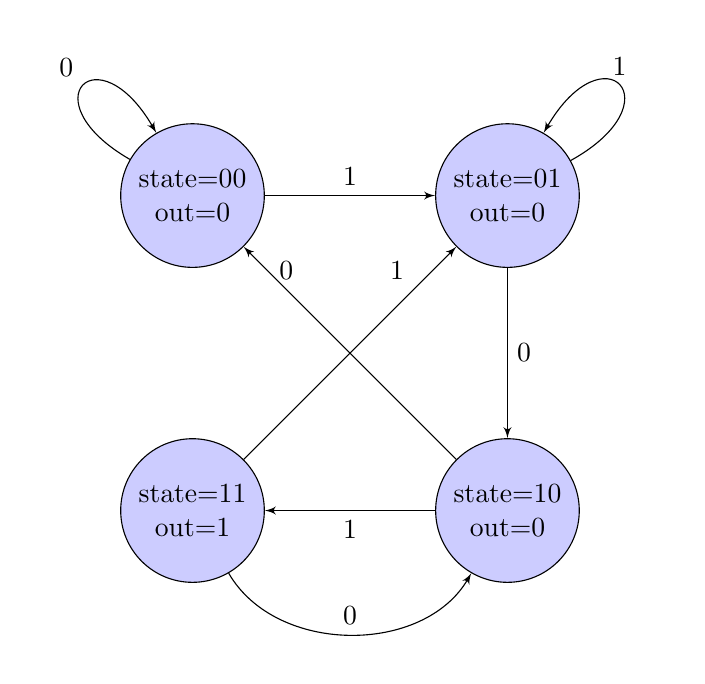
\begin{tikzpicture}[auto, node distance=4cm,>=latex',every text node
		part/.style={align=center}]
		\node[state] (zero) {state=00 \\ out=0};
		\node[state,right of=zero] (one) {state=01 \\ out=0};
		\node[state,below of=one] (two) {state=10 \\ out=0};
		\node[state,below of=zero] (three) {state=11 \\ out=1};

		\draw[->] (zero) to[out=150, in=120, looseness=8] node{0} (zero);	
		\draw[->] (one) to[out=29, in=60, looseness=8] node[above]{1} (one);	
		\draw[->] (one.south) -- node{0} (two.north);
		\draw[->] (zero.east) -- node{1} (one.west);
		\draw[->] (two.west) -- node{1} (three.east);
		\draw[->] (three) to[out=300,in=240] node{0} (two);
		\draw[->] (three.north east) -- node[pos=0.8]{1}(one.south west);
		\draw[->] (two.north west) -- node[pos=0.8,above]{0}(zero.south east);
	\end{tikzpicture}
	\caption{FSM A:	The \texttt{reset} signal should send the state machine back to
	state=00. The transition signal for this state machine is labeled
	\texttt{in}.}
\end{figure}

Fix the errors in this FSM (\texttt{fsm\_ab.v}) to operate as shown in Fig. 1.

\subsection{Part B}
\begin{figure}[H]
	\centering
	\begin{tikzpicture}[auto, node distance=4cm,>=latex',every text node
		part/.style={align=center}]
		\node[state] (wait) {state=WAIT \\ cnt+=0 \\ hit=0};
		\node[state,right of=zero,node distance=8cm] (watch) {state=WATCH \\ hit=0 \\
		if(seq==num) cnt++};
		\node[state,below of=watch] (assert) {state=ASSERT \\ cnt--\\ hit=1};

		\draw[->] (wait) to[out=150, in=120, looseness=6] node{!valid} (wait);	
		\draw[->] (watch) to[out=30, in=60, looseness=4] node[pos=0.6,node
		distance=3cm,above]{valid} (watch);	
		\draw[->] (assert) to[out=240, in=300, looseness=3] node[below]{cnt$>$1} (assert);	
		\draw[->] (assert).. controls+(180:5cm) and +(270:3cm) .. node{!(cnt$>$1)} (wait);
		\draw[->] (watch.south) -- node{n\_cnt!=0 \&\& !valid}(assert.north);
		\draw[->] (wait.30) -- node[above]{valid} (watch.160);
		\draw[->] (watch.west) -- node[below]{n\_cnt==0 \&\& !valid}
		(wait.east);
	\end{tikzpicture}
	\caption{FSM B:	The \texttt{reset} signal should send the state machine back
	to state=WAIT and set \texttt{cnt} to zero.}
\end{figure}

Fix the errors in this FSM (\texttt{fsm\_cd.v}) to operate as shown in Fig. 2.

\section{Submission}
Once you are confident in your module and testbench, put yourself on the \href{https://oh.eecs.umich.edu/courses/eecs470}{\underline{help queue}} and we will come check you off.

\end{document}
